%IEEE
\documentclass[conference, 12pt]{IEEEtran}
\usepackage{cite}
\usepackage{amsmath,amssymb,amsfonts}
\usepackage{algorithmic}
\usepackage{graphicx}
\usepackage{textcomp}
\usepackage{xcolor}
\usepackage{url}
\def\BibTeX{{\rm B\kern-.05em{\sc i\kern-.025em b}\kern-.08em
    T\kern-.1667em\lower.7ex\hbox{E}\kern-.125emX}}
\begin{document}

\title{Sockets}

\author{\IEEEauthorblockN{Davis Mariotti}
\IEEEauthorblockA{\textit{Computer Science Department} \\
\textit{Whitworth University}\\
Spokane, USA \\
dmariotti19@my.whitworth.edu}
\and
\IEEEauthorblockN{Michael Gamlem III}
\IEEEauthorblockA{\textit{Computer Science Department} \\
\textit{Whitworth University}\\
Spokane, USA \\
mgamlem19@my.whitworth.edu}
\and
\IEEEauthorblockN{Utsal Shrestha}
\IEEEauthorblockA{\textit{Computer Science Department} \\
\textit{Whitworth University}\\
Spokane, USA \\
ushrestha20@my.whitworth.edu}
}

\maketitle

\begin{abstract}
    Lorem ipsum dolor sit amet, consectetur adipiscing elit. Curabitur pellentesque mauris tellus, a facilisis metus congue et. Nullam gravida laoreet justo, auctor rutrum nibh porttitor nec. Suspendisse potenti. Nam in tincidunt nibh. Pellentesque habitant morbi tristique senectus et netus et malesuada fames ac turpis egestas. Morbi enim ex, dapibus efficitur lorem sit amet, maximus dictum eros. 
\end{abstract}

\begin{IEEEkeywords}
Socket, IP Address, Port, Pipelines
\end{IEEEkeywords}

\section{Introduction}
Modern computer networks rely on many technologies to function efficiently and effectively. The complex system is made of many smaller components each functioning to facilitate communication between two computer endpoints. Among the smaller components is the socket.

Non-common uses

It is attackable?

Can be used in creative ways

Is it the best?


\section{Definition}
A socket is not a physical piece of the computer, but rather, it is the idea that subdivisions can be made on the network interface to separate traffic and route it correctly to where it needs to go. A socket consists of an Internet Protocol (IP) address and a port number. It is commonly written in the form of 192.168.0.1:8080 \cite{6}. Some port numbers, such as 80 and 443, are reserved for specific applications or communication types while others are free for application programmers to utilize. Both IP Addresses and port numbers are “managed” by many local organizations, however the \url{https://www.iana.org/}{Internet Assigned Numbers Authority} (IANA) is commonly regarded as one of the most accurate authority for reference purposes.

\section{Uses}
Lorem ipsum dolor sit amet, consectetur adipiscing elit. Curabitur pellentesque mauris tellus, a facilisis metus congue et. Nullam gravida laoreet justo, auctor rutrum nibh porttitor nec. Suspendisse potenti. Nam in tincidunt nibh. Pellentesque habitant morbi tristique senectus et netus et malesuada fames ac turpis egestas.

\subsection{General Programming}
Lorem ipsum dolor sit amet, consectetur adipiscing elit. Curabitur pellentesque mauris tellus, a facilisis metus congue et. Nullam gravida laoreet justo, auctor rutrum nibh porttitor nec. Suspendisse potenti. Nam in tincidunt nibh. Pellentesque habitant morbi tristique senectus et netus et malesuada fames ac turpis egestas. Morbi enim ex, dapibus efficitur lorem sit amet, maximus dictum eros.

\subsection{Interprocess Communication}
Lorem ipsum dolor sit amet, consectetur adipiscing elit. Curabitur pellentesque mauris tellus, a facilisis metus congue et. Nullam gravida laoreet justo, auctor rutrum nibh porttitor nec. Suspendisse potenti. Nam in tincidunt nibh. Pellentesque habitant morbi tristique senectus et netus et malesuada fames ac turpis egestas. Morbi enim ex, dapibus efficitur lorem sit amet, maximus dictum eros.

\subsection{Internet Applications}
Lorem ipsum dolor sit amet, consectetur adipiscing elit. Curabitur pellentesque mauris tellus, a facilisis metus congue et. Nullam gravida laoreet justo, auctor rutrum nibh porttitor nec. Suspendisse potenti. Nam in tincidunt nibh. Pellentesque habitant morbi tristique senectus et netus et malesuada fames ac turpis egestas. Morbi enim ex, dapibus efficitur lorem sit amet, maximus dictum eros. 

\subsection{Distributed Computing}
Lorem ipsum dolor sit amet, consectetur adipiscing elit. Curabitur pellentesque mauris tellus, a facilisis metus congue et. Nullam gravida laoreet justo, auctor rutrum nibh porttitor nec. Suspendisse potenti. Nam in tincidunt nibh. Pellentesque habitant morbi tristique senectus et netus et malesuada fames ac turpis egestas. Morbi enim ex, dapibus efficitur lorem sit amet, maximus dictum eros. 

\section{Master/Slave Relationships}
Lorem ipsum dolor sit amet, consectetur adipiscing elit. Curabitur pellentesque mauris tellus, a facilisis metus congue et. Nullam gravida laoreet justo, auctor rutrum nibh porttitor nec. Suspendisse potenti. Nam in tincidunt nibh. Pellentesque habitant morbi tristique senectus et netus et malesuada fames ac turpis egestas. Morbi enim ex, dapibus efficitur lorem sit amet, maximus dictum eros. 

\section{Security}
As with most aspects of the internet today, security is an issue that cannot be ignored when discussing web sockets. Even though the standard has been around for decades, it has not been reliably or adequately updated to protect against modern security threats. This is due to many complicating factors that are outside the scope of this paper. However, below are some examples of both commonly exploited and uncommonly exploited vulnerabilities in the socket communication protocol as well as potential experimental solutions.

\subsection{Vulnerabilities}
There is no security built into the socket protocol. This means that all applications that use sockets must be designed to protect against any and all possible attack vectors. Some protections are given by host operating systems, however they are not all-inclusive and not always sufficient.

\subsubsection{No Built-In Security Measures}
There is no security built into the socket protocol. This means that all applications that use sockets must be designed to protect against any and all possible attack vectors. Some protections are given by host operating systems, however they are not all-inclusive and not always sufficient. This results in inconsistent security practices among applications who utilize sockets and an inability to quickly fix a security problem as many organizations must act separately to solve any security concerns.

At the Black Hat conference of 2009 a security researcher gave a presentation where they showed how simple it was to intercept Secure Socket Layer (SSL) traffic and compromise a user’s secret login data by performing a man-in-the-middle style attack\cite{17}. This traffic would be traveling across a socket from the user’s machine to the login server. Due to the fact that information traveling over sockets is not encrypted or otherwise protected by default. This researcher was able capture essentially all data that users were entering to the compromised website.

The attack was only able to be carried out when users were moving from an unsecured http page to a secured https page to log into the compromised service. The researcher was then able to intercept and reroute traffic to their proxy server before directing the traffic to its original destination\cite{17}. If the socket protocol included ways to verify that traffic had not been intercepted on its way to a destination or encrypted all information sent over a socket by default, this attack would not be able to be carried out.

\subsubsection{Blind Trust}
Due to the fact that operating systems protect I/O devices from being directly accessed by applications, applications must trust that the host operating system is delivering data exactly as it appeared over the socket\cite{15}. This is typically not an issue, however in cases where the host operating system has been taken over by a malicious entity or otherwise compromised, problems quickly arise.

Traditional computers and operating systems have no workable solution to this problem. Therefore, a new type of computer operating system called Proxos was developed by researchers at the University of Toronto with the specific goal of addressing this blind trust problem.

\begin{figure}[htbp]
    \centering
    \centerline{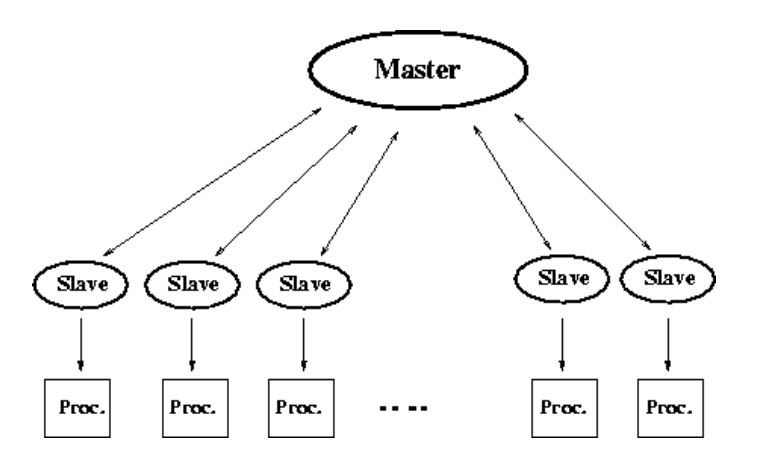
\includegraphics[width=0.5\textwidth]{Figure1.png}}
    \caption{Diagram of the Proxos System Architecture\cite{15}}
    \label{Figure1}
\end{figure}

As can be seen in the above figure, this system architecture is made up of three or more Virtual Machines (VM). The Virtual Machine Master (VMM) would be responsible for overseeing all other virtual machines that operate on the system. It would also be responsible for allocating resources to each VM as they are created or destroyed\cite{15}. It is not a traditional operating system. It is only intended to manage hardware resources and respond to requests made to those resources. The Commodity Operating System (OS), the researchers used Linux, would be what we are used to today, the traditional user operating system. It would be allowed to run application as any other normal operating system would. The only difference is that it is not responsible for handling hardware resources and can only ask the VMM for the resources it needs\cite{15}.

The main difference between Proxos and traditional computer systems lies in how it handles applications that want to have more security. These applications are given their own private VM with their own copy of the OS that can make trusted calls directly to the VMM and bypass a potentially compromised host operating system. Only the application is allowed in this private VM. Its application-trusted system calls are allowed to communicate directly with the VMM to get information directly from hardware resources……

\subsection{Potential Solutions}
Lorem ipsum dolor sit amet, consectetur adipiscing elit. Curabitur pellentesque mauris tellus, a facilisis metus congue et. Nullam gravida laoreet justo, auctor rutrum nibh porttitor nec. Suspendisse potenti. Nam in tincidunt nibh. Pellentesque habitant morbi tristique senectus et netus et malesuada fames ac turpis egestas. Morbi enim ex, dapibus efficitur lorem sit amet, maximus dictum eros. 

\section{Experimental Uses}
Lorem ipsum dolor sit amet, consectetur adipiscing elit. Curabitur pellentesque mauris tellus, a facilisis metus congue et. Nullam gravida laoreet justo, auctor rutrum nibh porttitor nec. Suspendisse potenti. Nam in tincidunt nibh. Pellentesque habitant morbi tristique senectus et netus et malesuada fames ac turpis egestas. Morbi enim ex, dapibus efficitur lorem sit amet, maximus dictum eros. 

\section{Comparison}
Lorem ipsum dolor sit amet, consectetur adipiscing elit. Curabitur pellentesque mauris tellus, a facilisis metus congue et. Nullam gravida laoreet justo, auctor rutrum nibh porttitor nec. Suspendisse potenti. Nam in tincidunt nibh. Pellentesque habitant morbi tristique senectus et netus et malesuada fames ac turpis egestas. Morbi enim ex, dapibus efficitur lorem sit amet, maximus dictum eros. 

\subsection{Pipes}
Lorem ipsum dolor sit amet, consectetur adipiscing elit. Curabitur pellentesque mauris tellus, a facilisis metus congue et. Nullam gravida laoreet justo, auctor rutrum nibh porttitor nec. Suspendisse potenti. Nam in tincidunt nibh. Pellentesque habitant morbi tristique senectus et netus et malesuada fames ac turpis egestas. Morbi enim ex, dapibus efficitur lorem sit amet, maximus dictum eros. 

\subsection{Remote Procedure Calls (RPC)}
Lorem ipsum dolor sit amet, consectetur adipiscing elit. Curabitur pellentesque mauris tellus, a facilisis metus congue et. Nullam gravida laoreet justo, auctor rutrum nibh porttitor nec. Suspendisse potenti. Nam in tincidunt nibh. Pellentesque habitant morbi tristique senectus et netus et malesuada fames ac turpis egestas. Morbi enim ex, dapibus efficitur lorem sit amet, maximus dictum eros. 

\section{Conclusion}
Lorem ipsum dolor sit amet, consectetur adipiscing elit. Curabitur pellentesque mauris tellus, a facilisis metus congue et. Nullam gravida laoreet justo, auctor rutrum nibh porttitor nec. Suspendisse potenti. Nam in tincidunt nibh. Pellentesque habitant morbi tristique senectus et netus et malesuada fames ac turpis egestas. Morbi enim ex, dapibus efficitur lorem sit amet, maximus dictum eros. Lorem ipsum dolor sit amet, consectetur adipiscing elit. Curabitur pellentesque mauris tellus, a facilisis metus congue et. Nullam gravida laoreet justo, auctor rutrum nibh porttitor nec. Suspendisse potenti. Nam in tincidunt nibh. Pellentesque habitant morbi tristique senectus et netus et malesuada fames ac turpis egestas. Morbi enim ex, dapibus efficitur lorem sit amet, maximus dictum eros. 

\begin{thebibliography}{00}
\bibitem{1}Arabo, Abdullahi. Distributed IDS using Agents: An Agent-Based Detection System to Detect Passive and Active Threats to a Network. Reading: Academic Conferences International Limited, 2019. ProQuest. Web. 10 Apr. 2019.
 
\bibitem{2}Bailey, Kimberly Tekavec. AF UNIX Socket Across Systems in the Same Computer on Computer Systems that Support Multiple Operating System Images. International Business Machines Corp, assignee. Patent US20080155103A1. 2008.
     
\bibitem{3}de, la C., et al. "Checking the Reliability of Socket Based Communication Software." International Journal on Software Tools for Technology Transfer 11.5 (2009): 359-74. ProQuest. Web. 10 Apr. 2019.
     
\bibitem{4}Ganger, Gregory R., et al. "Fast and Flexible Application-Level Networking on Exokernel Systems." ACM Transactions on Computer Systems 20.1 (2002): 49. ProQuest. Web. 10 Apr. 2019.
     
\bibitem{5}Gay, Warren W. “Linux Socket Programming: By Example”. Que Corp. Indianapolis, IN, USA, 2000.
     
\bibitem{6}Goralski, Walter. The Illustrated Network : How TCP/IP Works in a Modern Network, Elsevier Science \& Technology, 2008. ProQuest Ebook Central, \url{https://ebookcentral.proquest.com/lib/whitworth/detail.action?docID=405967}{https://ebookcentral.proquest.com/lib/whitworth/detail.action?docID=405967}.
     
\bibitem{7}Kalita, Limi. “Socket Programming”. International Journal of Computer Science and Information Technologies, Vol. 5 (3), 2014, 4802-4807.
     
\bibitem{8}Law, KL Eddie, and Roy Leung. "A design and implementation of active network socket programming." Microprocessors and Microsystems 27.5-6 (2003): 277-284.
     
\bibitem{9}Leffler, Samuel J., et al. “An Advanced 4.4BSD Interprocess Communication Tutorial”. University of California, Berkeley. 1986.
     
\bibitem{10}Matthew, Neil, and Richard Stones. Beginning linux programming. John Wiley \& Sons, 2008.
     
\bibitem{11}Mitchell, Mark, Jeffrey Oldham, and Alex Samuel. Advanced linux programming. New Riders Publishing, 2001.
     
\bibitem{12}Mohamed, Nader, et al. “A USER-LEVEL SOCKET LAYER OVER MULTIPLE PHYSICAL NETWORK INTERFACES.” ProQuest, University of Nebraska – Lincoln, \url{middleware-tech.net/papers/PDCS2002_IASTED_MuniSocket.pdf}.
     
\bibitem{13}Oliver, Stephen L., et al. “Scheduling task parallelism on multi-socket multicore systems”. Proceedings of the 1st International Workshop on Runtime and Operating Systems for Supercomputers. Tucson, Arizona, 2011, 49-56.
     
\bibitem{14}Reed, Dennis F., et al. “Interprocess communications system and method utilizing shared memory for message transfer and datagram sockets for message control”. US5652885A, United States Patent and Trademark Office. 1993.
     
\bibitem{15}Richard Ta-Min, Lionel Litty, and David Lie. 2006. Splitting interfaces: making trust between applications and operating systems configurable. In Proceedings of the 7th symposium on Operating systems design and implementation (OSDI '06). USENIX Association, Berkeley, CA, USA, 279-292.
     
\bibitem{16}Sawant, Abhijit A., and B. B. Meshram. "Network programming in Java using Socket." Network 3.1 (2013).
     
\bibitem{17}Sheble, Nicholas. "Black Hat Conference: Socket to Me." Intech 56.4 (2009): 9. ProQuest. Web. 10 Apr. 2019.
     
\bibitem{18}Stevens, W. Richard, and Stephen A. Rago. Advanced programming in the UNIX environment. Addison-Wesley, 2008.
     
\bibitem{19}Xue, Ming and Changjun Zhu. “The Socket Programming and Software Design for Communication Based on Client/Server”. 2009 Pacific-Asia Conference on Circuits, Communications and Systems. IEEE. 2009.    
\end{thebibliography}

\end{document}
